%% ----------------------------------------------------------------------
%% START OF FILE
%% ----------------------------------------------------------------------

\chapter{系统测试与结果分析}
\label{cha:exp_analysis}

\section{测试平台}
\label{sec:exp_platform}

操作系统 Microsoft Windows Server 2008 R2

机械硬盘 250GB seagate st9250320as

固态硬盘 120GB crucial ct120m500ssd1

驱动程序开发工具 Microsoft Windows Driver Kit 7600.1

应用程序开发工具 Microsoft Visual Studio 2008

\section{测试方法}
\label{sec:exp_method}

本缓存系统在Windows平台下实现,系统测试工作包括了正确性验证和性能测试两方面的评估。

\subsection{系统正确性验证}

使用Windows自带的chkdsk工具进行正确性验证,该工具用于检测保存在存储卷上的文件系统是否存在问题。测试前需要保证被测试的缓存卷本身不存在问题,最好的方法是使用系统自带的分区管理工具建立新存储卷用于测试。

验证步骤为:
\begin{enumerate}
\item 加载缓存驱动程序。
\item 开启对某个存储卷的缓存。
\item 使用性能测试工具测试读写性能。
\item 停止对存储卷的缓存。
\item 卸载缓存驱动程序。
\item 使用chkdsk检测被缓存的存储卷。
\end{enumerate}

如果最后一步chkdsk命令未检测出问题,说明缓存系统通过了正确性验证。

\subsection{系统性能测试}

\subsubsection{性能测试工具FIO}
FIO是一款基于GPLv2协议主要用于测试存储设备的性能和压力上限的存储器性能评测工具。除了存储设备,FIO还可测试CPU和NIC的IO性能。FIO支持13种不同的IO引擎,可以通过多线程或多进程模拟各种IO操作。作为一款开源工具,FIO支持几乎所有操作系统平台:Linux,FreeBSD,NetBSD,OS X,OpenSolaris,AIX以及Windows。

FIO只提供了命令行界面的用户交互方式。由于其提供了丰富可调的参数,FIO的可定制性非常强,可以根据测试者意图进行多种模式的测试。本系统测试工作也只使用了其中的一小部分。

\subsubsection{参数说明}

以下逐一介绍论文系统测试中所用到的各FIO选项,并对其参数加以说明。

\begin{lstlisting}
filename=\\\\.\\C:
\end{lstlisting}

filename参数指定需要进行测试的设备文件。论文实现的缓存系统以存储卷为单位,Windows操作系统只有将存储卷映射到某个的盘符(C、D、E……)后,才可进行访问。因此,对FIO来说要测试的存储设备指的就是某个盘符所映射的存储卷。

\begin{lstlisting}
size=2000MB
\end{lstlisting}

size参数指定待测试存储设备的空间大小,测试中机械硬盘存储卷空间为2000MB。一般来说,缓存大小设定为存储空间大小的5\%-15\%时缓存对系统IO性能提升的贡献最为明显,存在也最有意义。因此,测试中设定的缓存卷大小为200MB。使用Windows分区管理程序划分固态硬盘上的缓存卷。

\begin{lstlisting}
iodepth=8
\end{lstlisting}

iodepth参数用以设定测试中并发IO请求个数上限。应用程序通常使用同步和异步两种方式访问存储设备。以同步方式访问设备时,下一个IO请求要在上一个完成后才可进行,因此iodepth总是为1;异步方式访问,每次提交一批IO请求后等待这批请求的完成,以此减少交互次数,让设备有机会合并IO请求以进行并行处理。多进程操作系统内,绝大多数情况下访问设备的iodepth都大于1。

\begin{lstlisting}
numjobs=4
\end{lstlisting}

numjobs参数设定了同时进行的负载个数。每个线程可产生一个负载进行测试,numjobs指定了FIO同时启动的测试线程数目。

\begin{lstlisting}
blocksize=[4k, 16k, 64k]
\end{lstlisting}

blocksize参数设定IO请求的大小,即每次读写的存储块大小,默认值为4KB。测试中使用了4KB,16KB和64KB三种不同大小进行测试,以模拟不同应用场景下应用程序对于存储设备的读写请求,同时还可以评估可变长缓存块对系统性能的影响。

\begin{lstlisting}
rw=[randrw, randread, randwrite]
\end{lstlisting}

rw参数设定每次测试所产生的读写类型。FIO提供了顺序读、顺序写、混合顺序读写、随机读、随机写、混合随机读写六种读写类型,每次测试只能选择其中一种。由于不存在热数据,任何缓存系统对于顺序读写性能提升的效果都很有限,因此本论文不进行顺序读写的测试,只测试随机读、随机写和混合随机读写三种读写类型。

\begin{lstlisting}
runtime=1000
\end{lstlisting}

runtime参数设置FIO运行的时间上限,单位是秒。如果运行时间太短,测试结果受系统内其他进程影响的波动较大。经多次实验,测试时间长为1000秒时性能趋于稳定,测试结果最有说服力。

\begin{lstlisting}
random_distribution=zipf:1.2
\end{lstlisting}

random\_distribution参数设置测试中访问存储设备的访问分布模型。通过设置该参数,可以使某部分的访问概率比其他部分的大,而并非平均分散到各处,从而获得系统存在热数据的访问效果。默认参数下,测试中设备的访问位置完全随机,此时测试出的缓存性能无法体现出真实情况下热数据被频繁访问的效果,缓存命中率也不具有说服力。因此,本论文的测试中使用了齐夫分布(zipf)这种概率分布模型,齐夫分布是一种最常见的模拟热数据访问的概率模型,参数为1.2。

\section{测试结果}
\label{sec:exp_results}

chkdsk工具测试结果表明:论文实现的缓存系统正确性方面没有任何问题。下面主要对缓存系统的性能测试结果加以分析。

论文实现的缓存系统可运行于写穿(Write Through)和写回(Write Back)两种模式,每种模式下都进行了随机读、随机写和混合随机读写三种类型的测试。

\subsection{缓存命中率}

\begin{table}[H]
\centering
\caption{写回、写穿两种模式下的缓存命中率}
\begin{tabular}{|c|c|c|c|}
\hline
\diagbox{模式}{测试类型} & 随机读 & 随机写 & 混合随机读写 \\ 
\hline 写穿模式 & 70.27\% & 70.75\% & 70.61\% \\ 
\hline 写回模式 & 76.29\% & 76.43\% & 73.64\% \\ 
\hline 
\end{tabular} 
\label{tab:cache-hit-rate}
\end{table}

从上表可以看出,写回模式下缓存命的中率略高于写穿模式。写回模式下不定期的回写队列刷新操作,延长了数据在缓存中的停留时间,一定程度上提升了命中率。

\subsection{写穿(Write Through)模式下的测试结果}

\subsubsection{随机读速度测试}

\begin{table}[H]
\centering
\caption{随机读速度(KB/s,写穿法)}
\begin{tabular}{|c|c|c|c|}
\hline
\diagbox{块大小(KB)}{存储介质} & HDD & SSD & HDD with SSD Cache \\ 
\hline 4 & 417 & 19264 & 2063 \\ 
\hline 16 & 1651 & 59735 & 6319 \\ 
\hline 64 & 5810 & 142304 & 13203 \\ 
\hline 
\end{tabular} 
\label{tab:wt-rand-read-test}
\end{table}

写穿模式下,SSD缓存带来了2.3-4.9倍的HDD随机读性能提升。

\subsubsection{随机写速度测试}

\begin{table}[H]
\centering
\caption{随机写速度(KB/s,写穿法)}
\begin{tabular}{|c|c|c|c|}
\hline
\diagbox{块大小(KB)}{存储介质} & HDD & SSD & HDD with SSD Cache \\ 
\hline 4 & 1283 & 18620 & 1155 \\ 
\hline 16 & 5043 & 40634 & 4768 \\ 
\hline 64 & 16346 & 41615 & 15490 \\ 
\hline 
\end{tabular} 
\label{tab:wt-rand-write-test}
\end{table}

由于写穿模式下不缓存写操作,HDD的随机写性能略差于无缓存模式下的写性能。

\subsubsection{随机读写:读速度测试}

\begin{table}[H]
\centering
\caption{随机读写-读速度(KB/s,写穿法)}
\begin{tabular}{|c|c|c|c|}
\hline
\diagbox{块大小(KB)}{存储介质} & HDD & SSD & HDD with SSD Cache \\ 
\hline 4 & 420 & 14693 & 1590 \\ 
\hline 16 & 1657 & 46650 & 5327 \\ 
\hline 64 & 5598 & 105242 & 11929 \\ 
\hline 
\end{tabular} 
\label{tab:wt-randrw-read-test}
\end{table}

写穿模式下进行随机读写测试,SSD缓存带来了2.3-4.9倍的HDD随机读性能提升。

\subsubsection{随机读写:写速度测试}

\begin{table}[H]
\centering
\caption{随机读写-写速度(KB/s,写穿法)}
\begin{tabular}{|c|c|c|c|}
\hline
\diagbox{块大小(KB)}{存储介质} & HDD & SSD & HDD with SSD Cache \\ 
\hline 4 & 45 & 1688 & 181 \\ 
\hline 16 & 180 & 5427 & 616 \\ 
\hline 64 & 599 & 11925 & 1371 \\ 
\hline 
\end{tabular} 
\label{tab:wt-randrw-write-test}
\end{table}

写穿模式下进行随机读写测试,SSD缓存带来了2.4-4.0倍的HDD随机写性能提升。
理论上讲,工作在写穿模式下的缓存无法带来写操作的性能提升,上面的‘随机写速度’测试结果也说明了这点。混合随机读写测试之所以出现与之相悖的写性能提升效果,是因为混合随机读写模式下,读写请求交错存在于任务队列,而一部分读请求会在缓存中命中。这在一定程度上降低了机械硬盘的读写负载,间接导致随机写性能的相对提升。

\subsection{写回(Write Back)策略时的测试结果}

\subsubsection{随机读速度测试}

\begin{table}[H]
\centering
\caption{随机读速度(KB/s,写回法)}
\begin{tabular}{|c|c|c|c|}
\hline
\diagbox{块大小(KB)}{存储介质} & HDD & SSD & HDD with SSD Cache \\ 
\hline 4 & 417 & 19264 & 2970 \\ 
\hline 16 & 1651 & 59735 & 9821 \\ 
\hline 64 & 5810 & 142304 & 32857 \\ 
\hline 
\end{tabular} 
\label{tab:wb-rand-read-test}
\end{table}

写回模式下,SSD缓存带来了5.6-7.1倍的HDD随机读性能提升。

\subsubsection{随机写速度测试}

\begin{table}[H]
\centering
\caption{随机写速度(KB/s,写回法)}
\begin{tabular}{|c|c|c|c|}
\hline
\diagbox{块大小(KB)}{存储介质} & HDD & SSD & HDD with SSD Cache \\ 
\hline 4 & 1283 & 18620 & 3459 \\ 
\hline 16 & 5043 & 40634 & 8697 \\ 
\hline 64 & 16346 & 41615 & 21794 \\ 
\hline 
\end{tabular} 
\label{tab:wb-rand-write-test}
\end{table}

写回模式下,SSD缓存带来了1.3-2.6倍的HDD随机写性能提升。

\subsubsection{随机读写:读速度测试}

\begin{table}[H]
\centering
\caption{随机读写-读速度(KB/s,写回法)}
\begin{tabular}{|c|c|c|c|}
\hline
\diagbox{块大小(KB)}{存储介质} & HDD & SSD & HDD with SSD Cache \\ 
\hline 4 & 420 & 14693 & 2725 \\ 
\hline 16 & 1657 & 46650 & 8693 \\ 
\hline 64 & 5598 & 105242 & 27696 \\ 
\hline 
\end{tabular} 
\label{tab:wb-randrw-read-test}
\end{table}

写回模式下进行随机读写测试,SSD缓存带来了4.9-6.4倍的HDD随机读性能提升。

\subsubsection{随机读写:写速度测试}

\begin{table}[H]
\centering
\caption{随机读写-写速度(KB/s,写回法)}
\begin{tabular}{|c|c|c|c|}
\hline
\diagbox{块大小(KB)}{存储介质} & HDD & SSD & HDD with SSD Cache \\ 
\hline 4 & 45 & 1688 & 309 \\ 
\hline 16 & 180 & 5427 & 985 \\ 
\hline 64 & 599 & 11925 & 3221 \\ 
\hline 
\end{tabular} 
\label{tab:wb-randrw-write-test}
\end{table}

写回模式下进行随机读写测试,SSD缓存带来了5.3-6.8倍的HDD随机写性能提升。

\section{结果讨论}
\label{sec:results_and_comparation}

\subsection{HDD性能提升比例}

\begin{figure}[H]
\centering
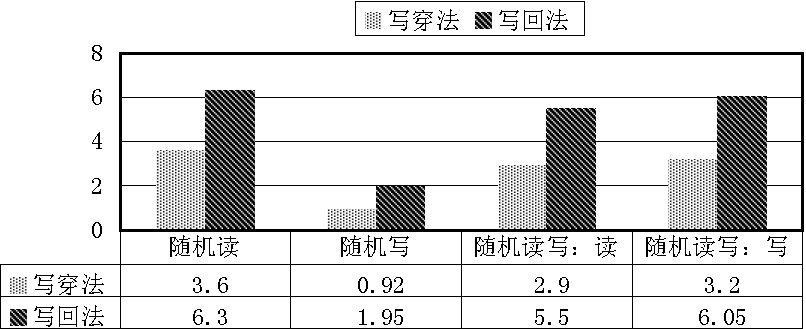
\includegraphics[width=0.9\linewidth]{./graph/enhance-rate}
\caption{读写性能提升比例比较}
\label{fig:enhance-rate}
\end{figure}

从图\ref{fig:enhance-rate}可以看出,缓存系统的存在从一定程度带来了HDD随机读、随机写的性能提升。相较于写穿法,写回法对存储系统的读写性能提升效果更为明显。

\subsection{与商业软件比较}

FancyCache是一款使用SSD作为缓存提升存储系统性能的商业软件。FancyCache可以将系统内存或SSD空间设置成机械硬盘的缓存。该软件的特点是,能够将从机械硬盘中读取的数据存入系统内存或闪存,避免下一次的访问发生在机械硬盘,从而提升IO性能突破硬盘瓶颈。FancyCache还能够通过特殊方式,识别并使用32位操作系统无法识别出的物理内存,解决32位Windows操作系统无法寻址4G以上内存的缺点。

为了说明本论文实现的缓存系统和FancyCache软件对性能提升的差距,系统的实验阶段在相同环境下测试了FancyCache软件对HDD的读写性能提升。由于本论文实现的缓存系统运行于回写模式时,对HDD的性能提升效果最为明显,且FancyCache软件只能运行于写回模式。因此,本节将使用运行于写回模式时的测试结果与FancyCache软件进行比较。

\begin{table}[H]
\centering
\caption{随机读速度比较(KB/s)}
\begin{tabular}{|c|c|c|}
\hline
\diagbox{块大小(KB)}{缓存系统} & 本论文的 & FancyCache \\ 
\hline 4  & 2970 & 2508 \\ 
\hline 16 & 9821 & 10254 \\ 
\hline 64 & 32857 & 51833 \\ 
\hline 
\end{tabular} 
\label{tab:wb-rand-read-comp}
\end{table}

随机读测试的结果表明,IO请求的大小为4KB时,本论文实现的缓存系统性能优于FancyCache;当IO请求比较大时,FancyCache的效果更为明显,这是因为论文实现的缓存系统中缓存块大小为4KB,读写请求大于4KB时需要将一个读写请求切分为多个处理,影响了系统的性能。

\begin{table}[H]
\centering
\caption{随机写速度比较(KB/s)}
\begin{tabular}{|c|c|c|}
\hline
\diagbox{块大小(KB)}{缓存系统} & 本论文的 & FancyCache \\ 
\hline 4  & 2970 & 3021 \\ 
\hline 16 & 9821 & 9982 \\ 
\hline 64 & 32857 & 32258 \\ 
\hline 
\end{tabular} 
\label{tab:wb-rand-write-comp}
\end{table}

随机写测试的结果表明,IO请求的大小为4KB和16KB时,FancyCache软件优于本论文实现的缓存系统,但差距不大;IO请求的大小为64KB时,本论文实现的缓存系统性能略优于FancyCache。

%% ----------------------------------------------------------------------
%%% END OF FILE
%% ----------------------------------------------------------------------
